\documentclass[a4paper,]{article}
\usepackage{lmodern}
\usepackage{amssymb,amsmath}
\usepackage{ifxetex,ifluatex}
\usepackage{fixltx2e} % provides \textsubscript
\ifnum 0\ifxetex 1\fi\ifluatex 1\fi=0 % if pdftex
  \usepackage[T1]{fontenc}
  \usepackage[utf8]{inputenc}
\else % if luatex or xelatex
  \ifxetex
    \usepackage{mathspec}
  \else
    \usepackage{fontspec}
  \fi
  \defaultfontfeatures{Ligatures=TeX,Scale=MatchLowercase}
\fi
% use upquote if available, for straight quotes in verbatim environments
\IfFileExists{upquote.sty}{\usepackage{upquote}}{}
% use microtype if available
\IfFileExists{microtype.sty}{%
\usepackage{microtype}
\UseMicrotypeSet[protrusion]{basicmath} % disable protrusion for tt fonts
}{}
\usepackage[margin=1in]{geometry}
\usepackage{hyperref}
\hypersetup{unicode=true,
            pdftitle={Closing the development gap between spatial modelling and onshore wind turbine acceptance rates},
            pdfauthor={Michael Harper, Ben Anderson, Patrick James, AbuBakr Bahaj},
            pdfborder={0 0 0},
            breaklinks=true}
\urlstyle{same}  % don't use monospace font for urls
\usepackage{longtable,booktabs}
\usepackage{graphicx,grffile}
\makeatletter
\def\maxwidth{\ifdim\Gin@nat@width>\linewidth\linewidth\else\Gin@nat@width\fi}
\def\maxheight{\ifdim\Gin@nat@height>\textheight\textheight\else\Gin@nat@height\fi}
\makeatother
% Scale images if necessary, so that they will not overflow the page
% margins by default, and it is still possible to overwrite the defaults
% using explicit options in \includegraphics[width, height, ...]{}
\setkeys{Gin}{width=\maxwidth,height=\maxheight,keepaspectratio}
\IfFileExists{parskip.sty}{%
\usepackage{parskip}
}{% else
\setlength{\parindent}{0pt}
\setlength{\parskip}{6pt plus 2pt minus 1pt}
}
\setlength{\emergencystretch}{3em}  % prevent overfull lines
\providecommand{\tightlist}{%
  \setlength{\itemsep}{0pt}\setlength{\parskip}{0pt}}
\setcounter{secnumdepth}{5}
% Redefines (sub)paragraphs to behave more like sections
\ifx\paragraph\undefined\else
\let\oldparagraph\paragraph
\renewcommand{\paragraph}[1]{\oldparagraph{#1}\mbox{}}
\fi
\ifx\subparagraph\undefined\else
\let\oldsubparagraph\subparagraph
\renewcommand{\subparagraph}[1]{\oldsubparagraph{#1}\mbox{}}
\fi

%%% Use protect on footnotes to avoid problems with footnotes in titles
\let\rmarkdownfootnote\footnote%
\def\footnote{\protect\rmarkdownfootnote}

%%% Change title format to be more compact
\usepackage{titling}

% Create subtitle command for use in maketitle
\newcommand{\subtitle}[1]{
  \posttitle{
    \begin{center}\large#1\end{center}
    }
}

\setlength{\droptitle}{-2em}
  \title{Closing the development gap between spatial modelling and onshore wind
turbine acceptance rates}
  \pretitle{\vspace{\droptitle}\centering\huge}
  \posttitle{\par}
  \author{Michael Harper, Ben Anderson, Patrick James, AbuBakr Bahaj}
  \preauthor{\centering\large\emph}
  \postauthor{\par}
  \date{}
  \predate{}\postdate{}

\usepackage{booktabs}
\usepackage{longtable}
\usepackage{array}
\usepackage{multirow}
\usepackage[table]{xcolor}
\usepackage{wrapfig}
\usepackage{float}
\usepackage{colortbl}
\usepackage{pdflscape}
\usepackage{tabu}
\usepackage{threeparttable}
\usepackage[normalem]{ulem}

\usepackage{setspace}\doublespacing

\usepackage{amsthm}
\newtheorem{theorem}{Theorem}[section]
\newtheorem{lemma}{Lemma}[section]
\theoremstyle{definition}
\newtheorem{definition}{Definition}[section]
\newtheorem{corollary}{Corollary}[section]
\newtheorem{proposition}{Proposition}[section]
\theoremstyle{definition}
\newtheorem{example}{Example}[section]
\theoremstyle{definition}
\newtheorem{exercise}{Exercise}[section]
\theoremstyle{remark}
\newtheorem*{remark}{Remark}
\newtheorem*{solution}{Solution}
\begin{document}
\maketitle

\subsection*{Abstract}\label{abstract}
\addcontentsline{toc}{subsection}{Abstract}

Geospatial modelling is extensively used to identify suitable sites for
the installation of onshore wind turbines. However, there are concerns
that such approaches do not accurately consider the social issues
surrounding such projects, resulting in large numbers of projects
subsequently being rejected at planning permission. Using the location
of 1691 wind turbine planning applications in Great Britain, this paper
explores whether the planning success of proposed wind turbine projects
can be predicted using a range of geospatial, social and political
parameters. The results indicate that the size of the project,
percentage of the local population with high levels of qualifications,
the average age, and local political composition emerge as key
influences affecting planning approval. The paper demonstrates that
quantitatively linking regional social and political data enhances the
assessment of the planning outcome of wind turbines, and highlights that
geospatial parameters are in themselves limited in identifying the
suitability of sites.

\subsection*{Keywords}\label{keywords}
\addcontentsline{toc}{subsection}{Keywords}

Onshore Wind, Logistic Regression, Planning, Demographics, Great
Britain, GIS

\textbf{Word Count}: 4306

\section{Introduction}\label{introduction}

Increased environmental concern and issues surrounding security of
energy supply have led to a global drive to develop renewable energy
systems. Onshore wind power generation is now competitive with fossil
energy in many countries and is one of the most mature renewable energy
technologies available {[}\protect\hyperlink{ref-UNEP2016}{1}{]}.
However, compared to other renewable energy technologies, onshore wind
turbine projects face significant difficulty in receiving planning
permission, with aesthetic perceptions often being the strongest single
influence on public attitudes
{[}\protect\hyperlink{ref-Wolsink2000}{2}{]}. Planning issues are
particularly visible within the UK, where 52\% of onshore wind projects
are refused permission or are abandoned by the developer
{[}\protect\hyperlink{ref-DECC2016}{3}{]}, a rate which is much higher
than other renewable energy technologies, as shown in Figure
\ref{fig:acceptanceRates}.

\begin{figure}[h]

{\centering 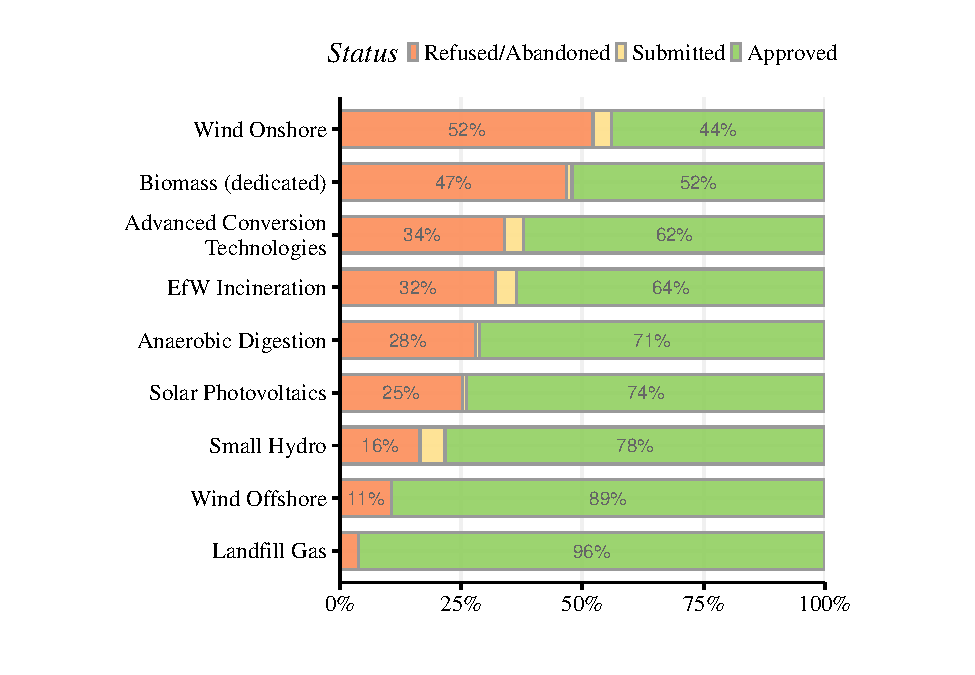
\includegraphics[width=8.8cm]{Wind_Stats_Paper_files/figure-latex/acceptanceRates-1} 

}

\caption{Acceptance rates of renewable energy projects within the UK between 1991 and 2017. Only considers technologies which have had more than 50 planning applications.}\label{fig:acceptanceRates}
\end{figure}

\subsection{Geospatial Modelling}\label{geospatial-modelling}

To assist in the development of onshore wind energy, many methodologies
have been produced to determine site suitability for wind farms.
Development primarily started within the late 1990s
{[}\protect\hyperlink{ref-Voivontas1998}{4},\protect\hyperlink{ref-Baban2001}{5}{]},
and established a structure which has been applied extensively
internationally
{[}\protect\hyperlink{ref-Hansen2005}{6}--\protect\hyperlink{ref-Baseer2017}{21}{]}.
These methodologies combine geospatial modelling with Multi-criteria
Decision Analysis (MCDA) techniques to identify sites which are deemed
suitable for development
{[}\protect\hyperlink{ref-Malczewski2004}{22}{]}.

When determining suitable sites for development, ideal sites are
typically identified as 1) \emph{having high average wind speeds};
\emph{2) not being close to urban areas}; \emph{3) not in protected
landscapes (e.g.~National Parks)}; \emph{4) not close to airports (to
minimise radar interference)}; \emph{5) close to roads for access} and
\emph{6) close to power lines for grid connection}. However, there are
concerns that geospatial parameters in isolation are in themselves
insufficient to explain patterns of development of wind turbines
{[}\protect\hyperlink{ref-VanderHorst2010}{23}{]}. These concerns can be
further supported by the continued reductions in the acceptance of wind
turbine projects in the UK, shown in Figure
\ref{fig:acceptanceRatesWind}, suggesting there is a widening gap
between existing modelling approaches and real world development
patterns.

\begin{figure}[h]

{\centering 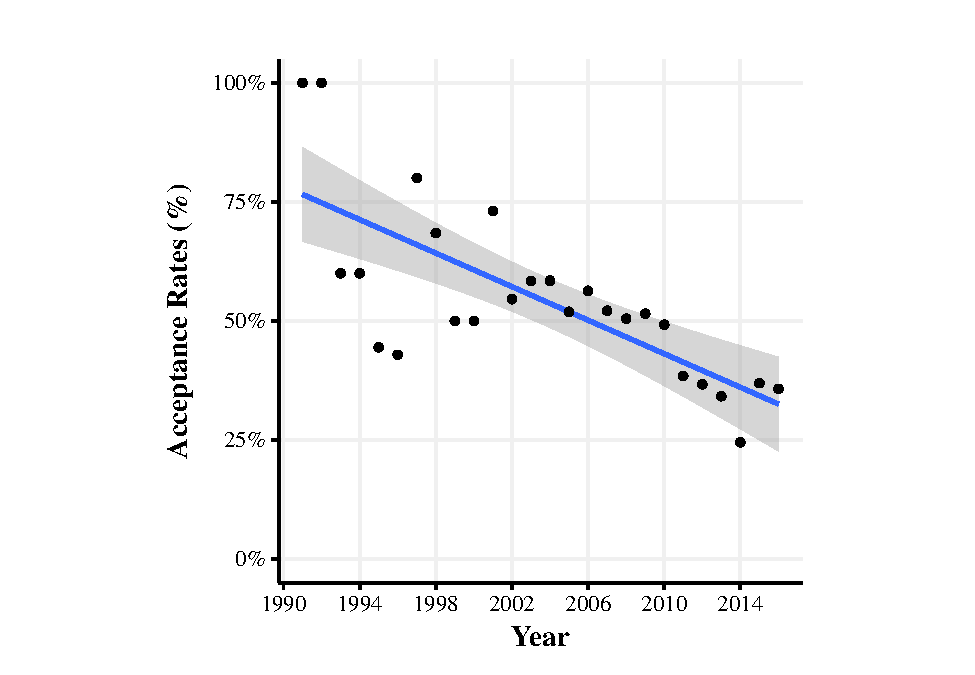
\includegraphics[width=8.8cm]{Wind_Stats_Paper_files/figure-latex/acceptanceRatesWind-1} 

}

\caption{Annual Average Acceptance rate of wind turbine projects within the UK}\label{fig:acceptanceRatesWind}
\end{figure}

Whilst some studies compare the resulting suitability maps with
locations of operational wind turbines
{[}\protect\hyperlink{ref-Aydin2010}{11},\protect\hyperlink{ref-VanHaaren2011}{12},\protect\hyperlink{ref-Gass2013}{14},\protect\hyperlink{ref-Miller2014}{16},\protect\hyperlink{ref-Watson2015}{18}{]},
these were largely used only as a form of discussion, and the
information was not directly used to develop or revise the models. This
overlooks a valuable contribution that existing sites could provide in
understanding whether there are any spatial development patterns which
can be identified. In particular, Watson
{[}\protect\hyperlink{ref-Watson2015}{18}{]} noted ``\emph{operational
wind farms in South Central England were predominantly located in areas
suggested to be of lower suitability}'', suggesting that the model is
inaccurately assessing site suitability in the region.

In situations where there is a large enough sample of similar historical
spatial decisions, an ``\emph{Inverse theory}'' approach can be applied
to determine subjective valuation of criteria by stakeholders
{[}\protect\hyperlink{ref-Cirucci2014}{24}{]}. Compared to the
traditional ``\emph{Forward theory}'' approach of geospatial modelling
(Fig \ref{fig:InverseGIS}a), an inverse approach assesses the existing
spatial distribution of projects to determine the most influential
parameters in determining site success (Fig. \ref{fig:InverseGIS}b).
Such an approach has been used successfully within public health studies
{[}\protect\hyperlink{ref-Brody2002}{25}--\protect\hyperlink{ref-Garcia-Ayllon2013}{28}{]}
and infrastructure location decision-making
{[}\protect\hyperlink{ref-USEPA2002}{29},\protect\hyperlink{ref-Cirucci2015}{30}{]}.

\begin{figure}[h]

{\centering 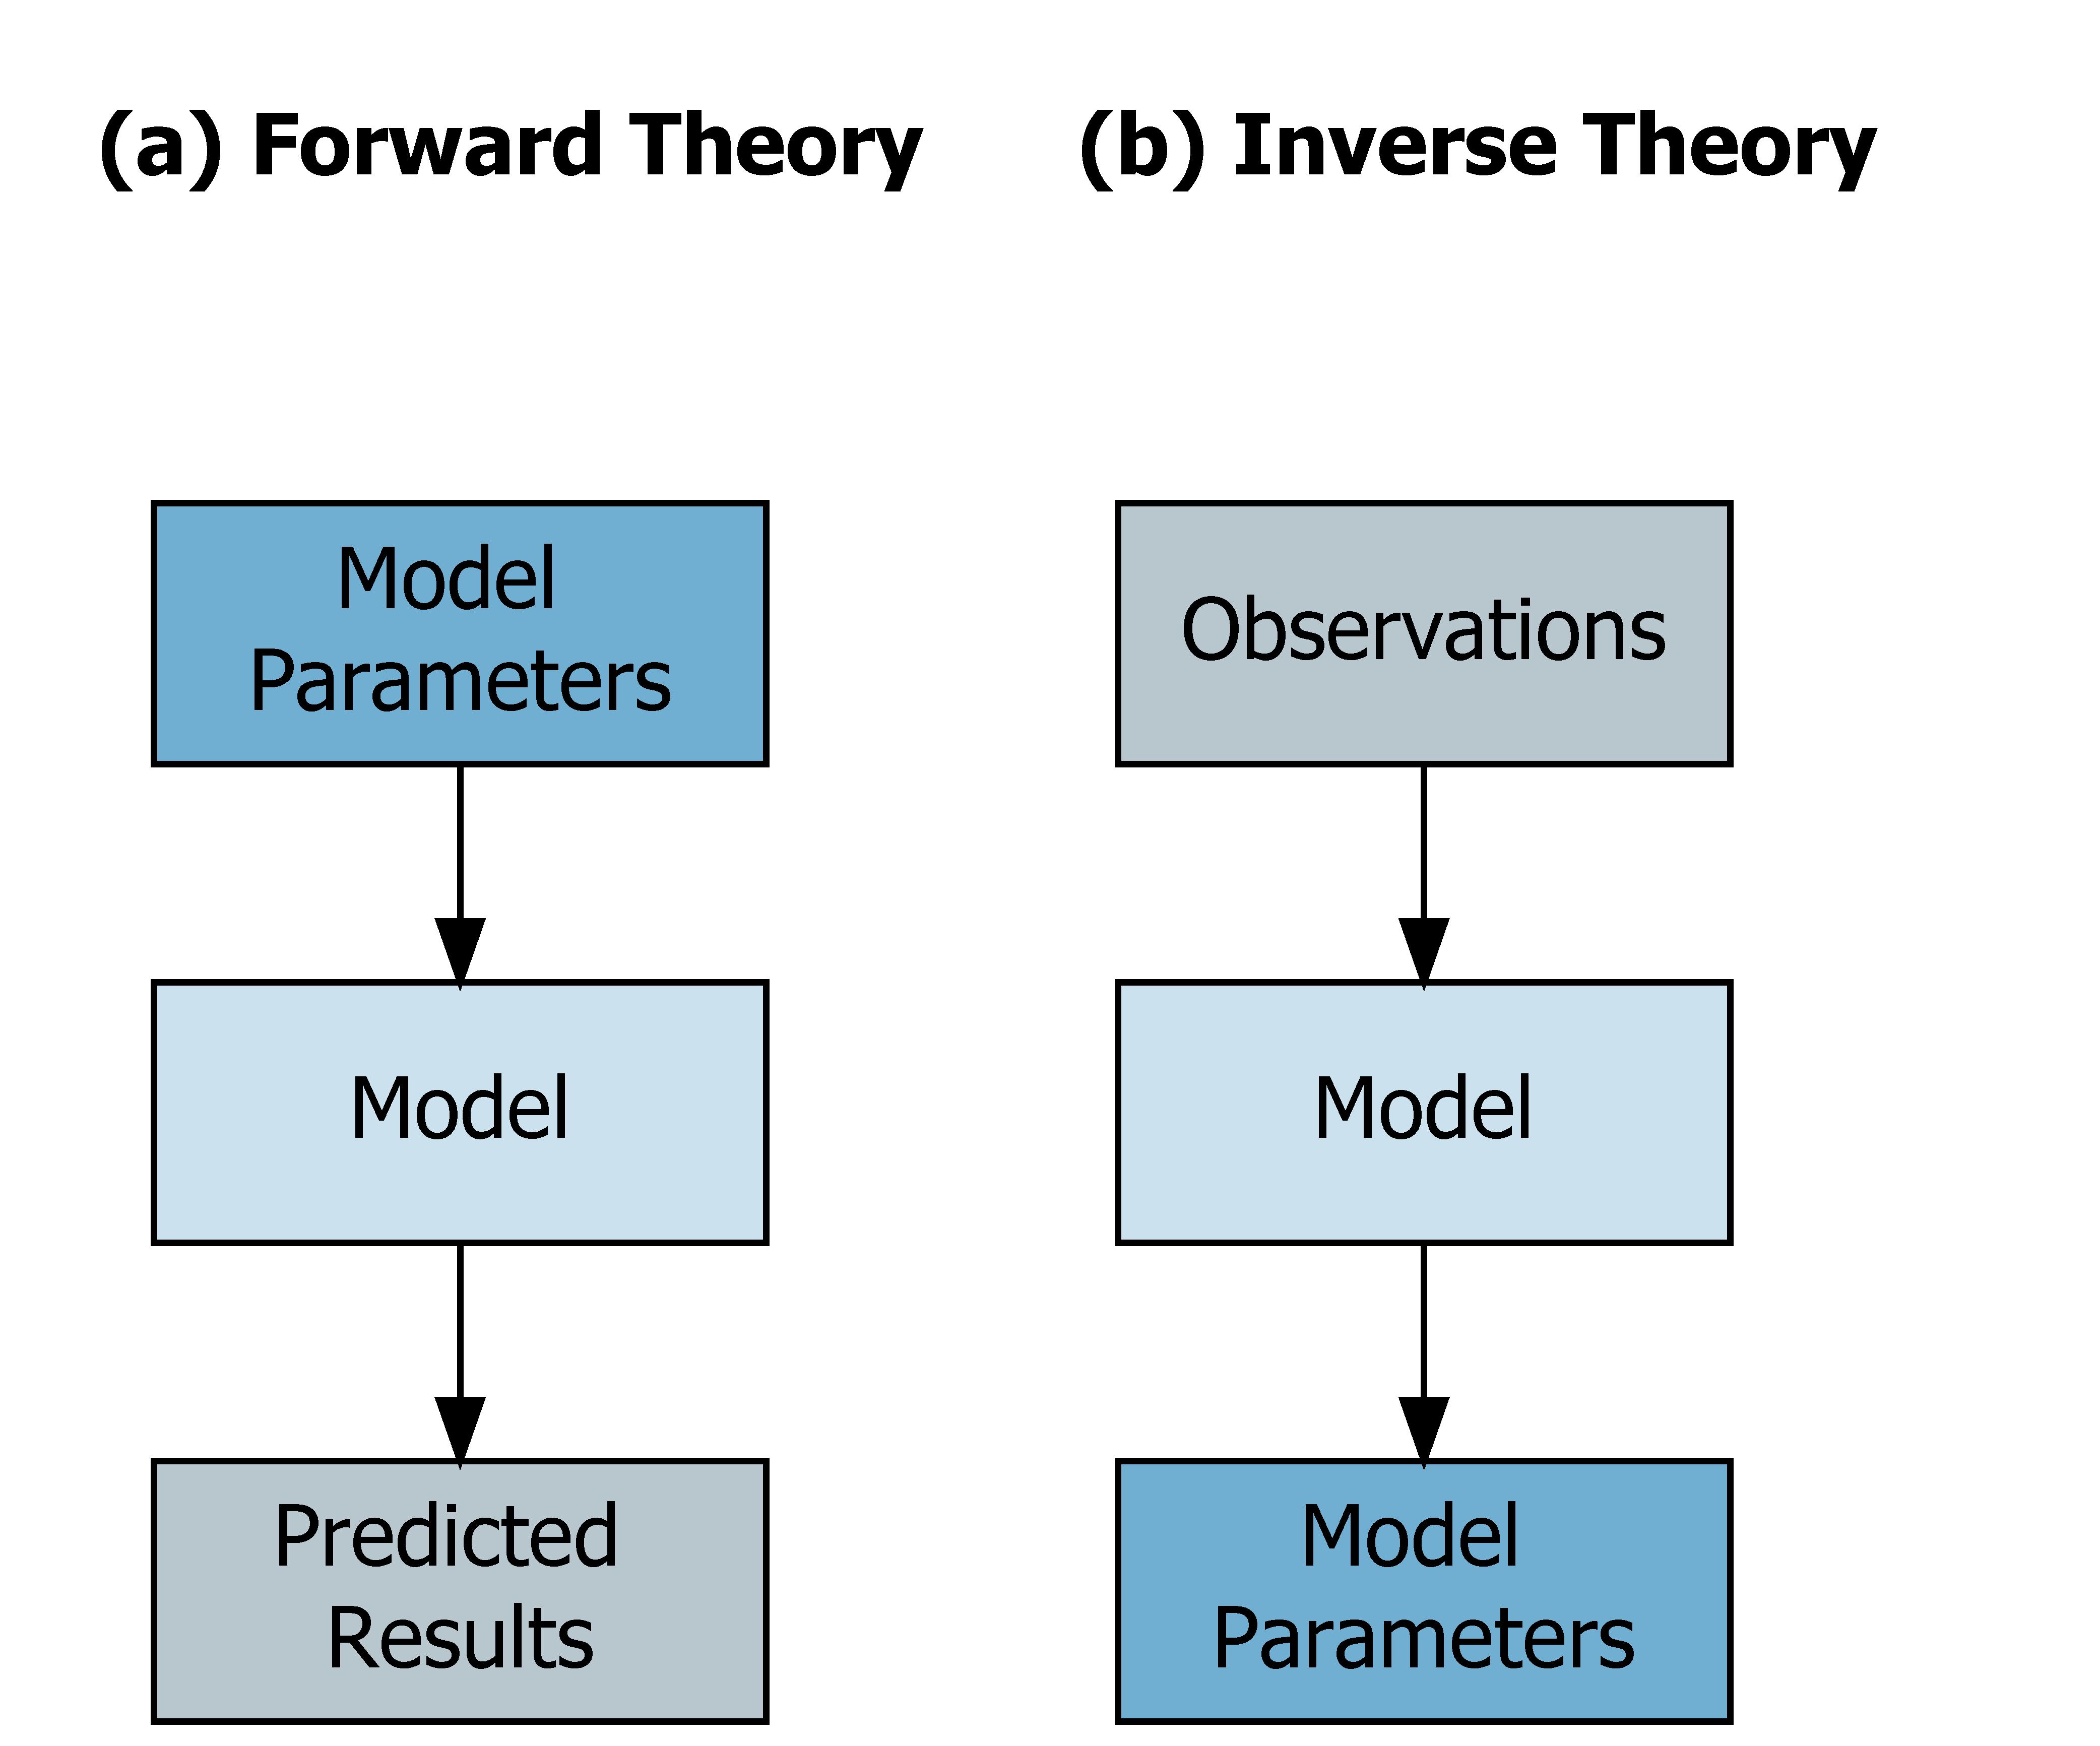
\includegraphics[width=0.5\linewidth]{figures/InverseGIS/InverseGIS} 

}

\caption{Comparison of Forward and Inverse GIS MCDA model structures}\label{fig:InverseGIS}
\end{figure}

\subsection{Planning Acceptance
Parameters}\label{planning-acceptance-parameters}

The difficulties in receiving planning permission for onshore wind
turbines has prompted research to assess the factors which influence the
public acceptance of onshore wind turbines. It has been highlighted that
the acceptability of wind energy projects is based on more than just
geospatial parameters
{[}\protect\hyperlink{ref-VanderHorst2010}{23},\protect\hyperlink{ref-Toke2008}{31},\protect\hyperlink{ref-Langer2016}{32}{]}.
In a review of 146 journal articles of planning acceptance, perceptions
and attitudes towards wind turbines, Langer et al
{[}\protect\hyperlink{ref-Langer2016}{32}{]} summarised that parameters
can be grouped into three groups 1): \emph{Physical and Environmental};
2) \emph{Pyscho-social} and 3) \emph{Social and Institutional}.

Qualatitive surveys are used to explore potential factors which
influence planning acceptance. A key concept consistently investigated
within empirical research is the \emph{``proximity hypothesis''}, which
states that those living closest to a wind farm will have the most
negative perceptions of it
{[}\protect\hyperlink{ref-Devine-Wright2005}{33},\protect\hyperlink{ref-Warren2005}{34}{]}.
However, attempts to prove this hypothesis have largely proved
unsuccessful, and results have proved conflicting. For example, evidence
from Denmark suggests no link between proximity of residential
properties to the nearest turbine and negative public perceptions, with
suggestions that respondents living closest (i.e.~within 500 metres)
actually had more positive perceptions in comparison with individuals
living away from turbines {[}\protect\hyperlink{ref-Krohn1999}{35}{]}.
This view was further supported by a study in Cornwall, UK, which found
that local communities with visibility of the turbines were generally
more supportive of wind turbines
{[}\protect\hyperlink{ref-Eltham2008}{36}{]}. However, several studies
have reported the opposite relationship
{[}\protect\hyperlink{ref-Meyerhoff2010}{37},\protect\hyperlink{ref-Ladenburg2006}{38}{]},
with the studies finding that negative perceptions increased with
proximity to wind energy developments.

Literature has also sought to understand the potential cumulative
effects that wind turbines have, as projects are frequently refused
planning in regions already containing wind turbines
{[}\protect\hyperlink{ref-Eltham2008}{36},\protect\hyperlink{ref-Strachan2004}{39},\protect\hyperlink{ref-Jones2011}{40}{]}.
However, there has been limited understanding in how neighbouring wind
energy projects may alter the likelihood of nearby wind turbine projects
receiving planning, and current research has focussed on smaller case
studies {[}\protect\hyperlink{ref-Jones2011}{40}{]}.\\
It has been argued within literature that psycho-social factors have
become crucial dimensions to explain how local communities interact
with, and react to, new wind farm developments
{[}\protect\hyperlink{ref-Langer2016}{32}{]}. The effects of
socio-demographic variables on individuals' views of wind farms have
also been studied within literature
{[}\protect\hyperlink{ref-Devine-Wright2005}{33},\protect\hyperlink{ref-Warren2010}{41}{]}.
Age, gender, experience with wind farms, and use of the land and/or
beach were found to be slightly correlated with the attitudes towards
wind power in a Danish study dealing with public perceptions of onshore
or offshore wind energy projects.

At an individual level, empirical findings suggest that political
beliefs are correlated with social acceptance of different low carbon
technologies {[}\protect\hyperlink{ref-Devine-Wright2007}{42}{]}. This
is supported by surveys that indicated that only 62\% of individuals
indicating support for the Conservative party were supportive of new
renewable energy developments, compared to 86\% and 84\% for Labour and
Liberal Democrats respectively
{[}\protect\hyperlink{ref-Populus2005}{43}{]}.

Studies have highlighted that the interaction of developers with local
communities are key indicators of positive planning approval outcomes
{[}\protect\hyperlink{ref-Toke2005}{44}--\protect\hyperlink{ref-Wustenhagen2007}{46}{]}.
Projects which seek greater approval within their plans are generally
more successful than those which are fixed prior to consultation with
the local population.

Finally, the ownership structure of a project has been indicated to be a
significant influence on the level of public acceptance
{[}\protect\hyperlink{ref-Sonnberger2017}{47},\protect\hyperlink{ref-Haggett2006}{48}{]}.
Projects are generally seen as more favourable when owned by local
energy cooperatives than by a large energy company or investor with no
local connections. This reason has been raised to explain the
differences in project success between the United Kingdom and Germany
{[}\protect\hyperlink{ref-Toke2008}{31}{]}.

\subsection{Quantitative Analysis of Turbine
Acceptance}\label{quantitative-analysis-of-turbine-acceptance}

There has been increased use of quantitative analysis to quantify the
effect parameters have on the outcome of wind energy planning outcomes.
Such approaches build upon the understandings provided within the
qualitative analysis explained with Section
\ref{planning-acceptance-parameters}, and aim to provide numerical data
that can be transformed into usable statistics.

Toke {[}\protect\hyperlink{ref-Toke2005}{44}{]} conducted logistic
regression analysis using data collected for 51 wind energy sites within
the UK, and explored how planning outcomes were influenced by the views
of key actors within the planning process of wind energy, including
local councils, planning authorities and landscape protection groups.
The study found that planning acceptance rates were closely associated
with the high level of apprehension about such schemes amongst people
living in the immediate vicinity, highlighting the importance that
social influences have on planning acceptance.

Van der Horst and Toke {[}\protect\hyperlink{ref-VanderHorst2010}{23}{]}
assessed how local characteristics related to the planning outcome of
wind energy projects in England. 117 variables related to education,
health, demography, employment and housing were used and compared with
the planning outcomes for 77 wind energy projects (of which 40 were
approved). Univariate regression analysis was conducted with the
Mann-Whitney test being used to analyse the associations between the
dependent variable (the planning decision outcome) and each of the
independent variables separately. Several strong associations were
identified for planning refusal, including (1) \emph{voter turnout} and
(2) \emph{years of potential life lost}\footnote{Years of potential life
  lost (YPLL) is an estimate of the average years a person would have
  lived if he or she had not died prematurely. It is, therefore, a
  measure of premature mortality.}. The study notes that wind energy
appears to generally be more likely to receive planning permission in
deprived areas, and as previously noted within the review, some
developers were ``\emph{keen to avoid relatively privileged communities
and target areas where people are thought to less likely put up a
fight}'' {[}\protect\hyperlink{ref-VanderHorst2010}{23}{]}. These issues
highlight the potential importance of social parameters in site
selection.

Van Rensburg et al. {[}\protect\hyperlink{ref-VanRensburg20}{49}{]}
utilised adjusted probit regression to assess the relative magnitudes of
association amongst wind farm project planning approval against a range
of 66 variables including project technology, institutional processes
and site endowment. Information was collected from 354 wind farm
applications and planning authority decisions between 1990 and 2011 in
Ireland. The results suggested a range of variables which appeared
significant for planning, including 1) \emph{proximity to Natura 2000
sites}; 2) \emph{sites with high bird sensitivity}; 3) \emph{hub height}
and 4) \emph{project capacity}. In addition, the study noted that
proximity of the nearest dwellings and wind speeds appeared
insignificant, which is counter to the view reported within many
previous studies. Of the variables included within the model, it
concluded a 0.31 predictive confidence value.

\subsection{Combining GIS and Quantitative
Research}\label{combining-gis-and-quantitative-research}

Whilst studies suggest a relationship between demographic and social
data and wind turbine planning acceptance rates, none of geospatial
models reviewed attempted to integrate these into their assessment
beyond the use of proximity buffers around urban areas. It is argued
that this omission fails to fully factor in the social dimension in
terms of its impact on the suitability of sites for development.

Existing quantitative studeis highlight the value which can be provided
by assessing previous planning applications. However, these projects
have been limited in the number of projects considered and the
parameters considered. Responding to calls to combine qualitative and
quantitative research {[}\protect\hyperlink{ref-Langer2016}{32}{]}, this
paper presents analysis which assesses parameters that influence wind
turbine planning outcomes, utilising a range of physical, geographical,
demographic and political parameters.

\section{Material and Methods}\label{material-and-methods}

The overall methodology is highlighted in Figure \ref{fig:Methodology},
with a detailed explanation provided in the following subsections.

\begin{figure}[h]

{\centering 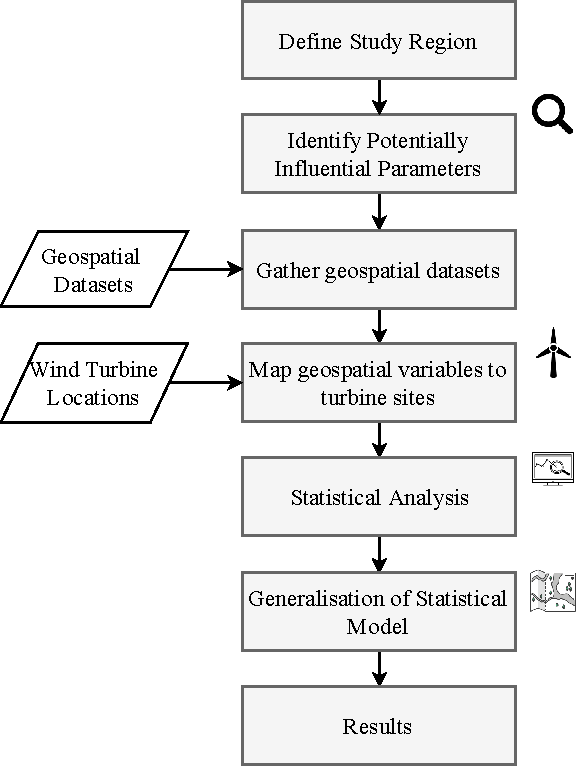
\includegraphics[width=8.8cm]{figures/Flowchart/ResearchApproach} 

}

\caption{Research methodology}\label{fig:Methodology}
\end{figure}

\subsection{Scope}\label{scope}

The study was conducted across Great Britain (England, Scotland \&
Wales). These were chosen due to the broadly similar categorisation of
land types, nature designation, data availability and legislation across
these regions {[}\protect\hyperlink{ref-HMGovernment2014}{50}{]}. The
Shetland Islands were excluded from the analysis as their geographic
isolation and distance from mainland Britain created issues in
generalising the model results.

\subsubsection{Wind Turbines Dataset}\label{wind-turbines-dataset}

Information for turbine planning applications was collected through the
Renewable Energy Planning Database (REPD)
{[}\protect\hyperlink{ref-DECC2016}{3}{]} with planning dates between
January 1991 and September 2017 (n=1755). Detailed information for each
planning application includes the location; year of application; number
of turbines; turbine capacity and planning decision. The planning
permission status was summarised to a dichotomous variable for use
within the statistical analysis: 1) \emph{Approved} and 2)
\emph{Refused/Abandoned}. The spatial distribution of these sites is
highlighted in Figure \ref{fig:StudyExtent}.

\begin{figure}[h]

{\centering 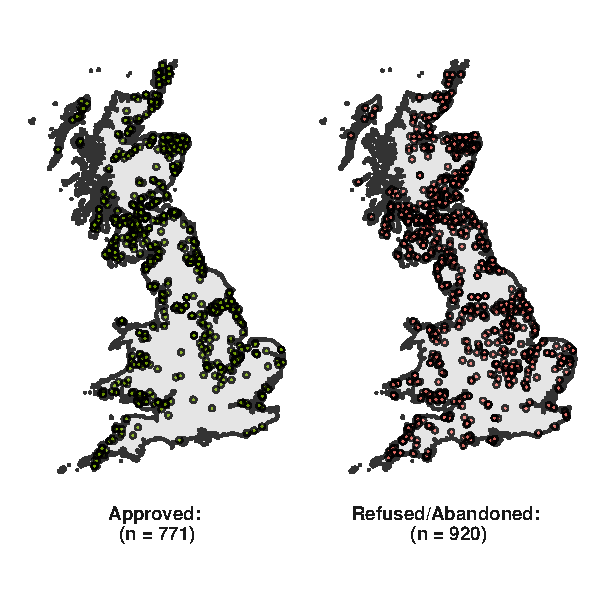
\includegraphics[width=8.8cm]{Wind_Stats_Paper_files/figure-latex/StudyExtent-1} 

}

\caption{Location of onshore wind energy planning applications used within the study. Location data extracted from the Renewable Energy Planning Database (REPD)}\label{fig:StudyExtent}
\end{figure}

\subsubsection{Model Layers Data}\label{model-layers-data}

Building upon the literature referenced in Section \ref{introduction},
data sources were identified for geospatial and social parameters which
had been indicated to be influence wind turbine planning applications. A
summary of the variables is provided in Table \ref{tab:SummaryTable},
with a full details provided within the Technical Appendix A.

\begin{table}

\begin{threeparttable}
\caption{\label{tab:SummaryTable}Parameters considered within model}
\centering
\begin{tabular}[t]{ll}
\toprule
Category & Variable\\
\midrule
Turbine & Wind Turbine Planning Data\\
 & Turbine Capacity\\
 & Number of Turbines\\
 & Year\\
 & Country\\
Resource & Wind Speed\\
Features & Airports\\
 & Roads\textsuperscript{a}\\
 & Railways\\
 & Urban Areas\\
 & HV Powerlines\textsuperscript{b}\\
Landscape & Areas of Outstanding Natural Beauty\\
 & National Parks\\
 & Heritage Coast\\
Nature & Special Protection Areas\\
 & National Nature Reserve\\
 & Sites of Special Scientific Interest\\
 & Special Areas of Conservation\\
Geographic & Elevation\\
 & Slope\\
Census & Level of Qualification\textsuperscript{c}\\
 & Age\\
 & Social Grade\textsuperscript{d}\\
 & Tenure\\
Political & Conservatives\\
 & Labour\\
 & Liberal Democrat\\
Proximity & Nearest Turbine (Operational)\\
 & Nearest Turbine (Rejected)\\
\bottomrule
\end{tabular}
\begin{tablenotes}
\small
\item[a] Roads are broken into four main categories: Motorways, A Roads, B Roads and Minor Roads
\item[b] High Voltage network at 140 400kV
\item[c] L4 represents degree level or above
\item[d] AB represents Higher and intermediate managerial, administrative, professional occupation
\end{tablenotes}
\end{threeparttable}
\end{table}

\begin{itemize}
\tightlist
\item
  \textbf{Resource}: wind speeds were taken from the Numerical Objective
  Analysis of Boundary Layer (NOABL) wind speed database. This provides
  estimated annualised wind speed at 45m elevation at a resolution of
  1km grid {[}\protect\hyperlink{ref-DTI2001}{51}{]}, and has been used
  in previous studies within the UK
  {[}\protect\hyperlink{ref-Baban2001}{5},\protect\hyperlink{ref-Watson2015}{18}{]}.
\item
  \textbf{Features}: Physical features including roads, railways and
  urban areas were collected from OS Strategi
  {[}\protect\hyperlink{ref-Survey2016}{52}{]}. The electricity
  transmission network, military sites and airport locations (civil and
  military) were extracted from Open Street Maps (OSM)
  {[}\protect\hyperlink{ref-Overpass2016}{53}{]}.
\item
  \textbf{Landscape and Nature}: Landscape and nature designations were
  collected for regions within the UK
  {[}\protect\hyperlink{ref-Pope2017}{54}{]}.
\item
  \textbf{Geographic}: Site elevation data was collected at a 25m
  resolution {[}\protect\hyperlink{ref-Commission2015}{55}{]}. This was
  used to calculate the gradient using the Fleming and Hoffer algorithm
  {[}\protect\hyperlink{ref-Fleming1979}{56}{]}.
\item
  \textbf{Census}: Census data was collected at the Lower Super Output
  Area (LSOA) and Data Zone (Scotland) which represents regions with a
  population between 1000 and 3000 people
  {[}\protect\hyperlink{ref-OfficeforNationalStatistics}{57}{]}.\\
\item
  \textbf{Political}: Political data was collected at the local
  authority level for the four largest parties in the UK: 1)
  \emph{Conservatives}; 2) \emph{Labour}, 3) \emph{Liberal Democrat} and
  4) - \emph{Scottish National Party (SNP)}. These parties hold a sum of
  95\% of council seats within Great Britain as of 2016.
\item
  \textbf{Cumulative}: the nearest wind turbine to the project was
  calculated using the location and year of planning application for
  each turbine.
\end{itemize}

Despite efforts to collect as many datasets as possible, there were
difficulties in collecting several features:

\begin{itemize}
\tightlist
\item
  \textbf{Bird Mapping}:
\end{itemize}

\subsection{Data Transformations}\label{data-transformations}

The data sources came in a range of formats including points, lines and
polygons (roads, urban regions etc.), tabular (census and political
data) and rasters (wind speed, elevation, slope). These parameters had
to be summarised for each wind turbine farms within the model, as
follows:

\begin{itemize}
\tightlist
\item
  \textbf{Points, lines and polygons}: A spatial join was completed to
  find the distance to the nearest feature for each turbine. For polygon
  based data source, value of 0km denotes the turbine is within the
  feature. Left censoring was used to limit the maximum distance of
  geospatial relationships to 30km, preventing extreme values from
  skewing the datasets.
\item
  \textbf{Tabular}: corresponding political and census boundaries were
  used to map the tabular data, and turbines assigned the value of the
  region. In addition, political data was filtered to the year of the
  planning application to determine the political balance at the time of
  planning.
\item
  \textbf{Raster}: The raster value at the site location was extracted.
\end{itemize}

\subsection{Statistical Modelling}\label{statistical-modelling}

A multiple logistic regression analysis was conducted to model the
factors associated with a positive planning outcome of wind turbine
applications using the predictor variables listed in Table
\ref{tab:ModelsSummary}. This model built upon the approaches developed
by Toke et al. {[}\protect\hyperlink{ref-Toke2005}{44}{]} and Van
Rensburg et al. {[}\protect\hyperlink{ref-VanRensburg20}{49}{]}. A
hierarchical approach was applied to the model whereby parameters are
added to the model sequentially based on the presumed importance of
parameters. These were selected as follows:

\begin{enumerate}
\def\labelenumi{\arabic{enumi}.}
\tightlist
\item
  \textbf{Aspatial Site Attributes}: variables including \emph{Number of
  Turbines} and \emph{Installed Capacity}.
\item
  \textbf{Economic Considerations}: parameters which influence the cost
  effectiveness of the site, including \emph{Wind Speed} and
  \emph{Proximity to the National Grid}.
\item
  \textbf{Temporal Aspect}: the year in which the planning application
  was made.
\item
  \textbf{Proximity to Features}: proximity to geographic features,
  Landscape and Nature Designations
\item
  \textbf{Social and Census Data}: Demographic data for the area of the
  wind energy project
\item
  \textbf{Political Data}: the political composition of the local
  authority composition at the time of the planning application.
\item
  \textbf{Spatial Proximity to Other Turbines}: the proximity to the
  nearest wind energy project.
\end{enumerate}

For each additional set of parameters added to the model, diagnostic
checks were made to ensure that the assumptions of logistic regression
were maintained. Each parameter was checked for linearity of the logit
for independent variables, absence of multicollinearity and independence
of variables {[}\protect\hyperlink{ref-Harrell2001}{58}{]}. Any
parameters which violated these conditions were removed from the model.
The overall fit of the model was assessed using Pearson chi-squared,
Psuedo R\textsuperscript{2} values and the residual deviance. Internal
validation was used to assess the predictive accuracy of the model
{[}\protect\hyperlink{ref-Hosmer2004}{59}{]}. Once all parameters had
been included within the model, a parsimonious model was produced to
remove uninfluential parameters, with the Akaike Information Criterion
(AIC) used to determine the best fitting model.

Regional differences in parameters effects between England, Scotland and
Wales were hypothesised due to differing population densities (England:
413/km\textsuperscript{2}, Wales: 149/km\textsuperscript{2}, Scotland:
68/km\textsuperscript{2}) {[}\protect\hyperlink{ref-ONS2013}{60}{]} as
well as differing institutional support, with Scotland in particular
placing a greater emphasis on the development of onshore wind {[}46{]}.
To test this, separate logistic regression models were produced for each
country. These included the key parameters identified within the
parsimonious model, with the additional inclusion of Wind Speed, which
had been suggested to be influential in previous research
{[}\protect\hyperlink{ref-VanRensburg20}{49}{]}.

\subsection{Generalisation}\label{generalisation}

Spatial regression models can be used to generalise the findings of
statistical analysis, and are frequently used within geospatial
modelling {[}\protect\hyperlink{ref-Ward2008}{61}{]}. The parsimonious
regression model was used to generalise the results for national
prediction. This model contained \texttt{13} variables, two of which
were non-spatial parameters, \emph{Turbine Capacity} and \emph{Year}. To
include these within the prediction, fixed values were assumed, with a
Turbine Size of 2MW (the average size of wind turbines in 2016 as shown
in Section \ref{TurbineSize}) and predictions made for the year 2017.

\section{Results}\label{results}

Table \ref{tab:LogisticResults} provides the results from the
parsimonious logistic regression analysis associating planning approval
for all available cases. Statistically significant positive trends
(e.g.~increase in the parameter increases success rates) were observed
for Number of Turbine; Distance to Urban Regions; Distance to National
Parks; Percentage of local council Liberal Democrat and Percentage of
local council Labour. Negative associations were found for
Qualifications above L4 (university degree); Mean Age and Distance to
Natura 2000 sites. The odds ratios (OR) are shown for each parameter in
Figure 4, whereby an OR = 1 means the parameter does not affect odds of
the planning outcome, OR \textgreater{} 1 indicate the parameters
positively influence planning acceptance, OR \textless{} 1 represents a
negative parameter influence.

As noted, the reduced parameter set of parameters were also used to
assess models for England, Scotland and Wales separately and the odds
ratios for each parameter for these models are shown in Figure
\ref{fig:OddsPlotSegmented}. The split logistic regression models are
summarised in Table \ref{tab:ModelsSummary}.

\begin{table}

\caption{\label{tab:LogisticResults}Logistic Regression results for the AIC optimised model.}
\centering
\begin{tabular}[t]{lrrrlrrr}
\toprule
Variable & Estimate & Std. Error & Pr & Sig. & Odds Ratio & 2.50\% & 97.50\%\\
\midrule
(Intercept) & 1.675 & 0.755 & 0.027 & * & 5.337 & 1.220 & 23.596\\
Number of Turbines & 0.017 & 0.007 & 0.010 & ** & 1.018 & 1.005 & 1.032\\
Distance to  Urban Region & 0.158 & 0.051 & 0.002 & ** & 1.171 & 1.060 & 1.295\\
Distance to National Park & 0.008 & 0.002 & 0.000 & *** & 1.008 & 1.005 & 1.011\\
Distance to Ramsar & 0.007 & 0.004 & 0.089 & . & 1.007 & 0.999 & 1.014\\
\addlinespace
Distance to SPA & -0.013 & 0.006 & 0.041 & * & 0.987 & 0.974 & 0.999\\
Qualifications, L4 & -0.036 & 0.007 & 0.000 & *** & 0.965 & 0.952 & 0.978\\
Mean Age & -0.043 & 0.016 & 0.006 & ** & 0.958 & 0.928 & 0.988\\
Political, Labour Share & 0.009 & 0.003 & 0.001 & *** & 1.009 & 1.004 & 1.015\\
Political, Liberal Democrat & 0.009 & 0.004 & 0.030 & * & 1.009 & 1.001 & 1.017\\
\bottomrule
\end{tabular}
\end{table}

\begin{table}[!h]

\caption{\label{tab:LogisticModelComparison}A summary of the hierarchical logistic regression models}
\centering
\resizebox{\linewidth}{!}{\begin{tabular}[t]{llllllll}
\toprule
 & Model 1 & Model 2 & Model 3 & Model 4 & Model 5 & Model 6 & Model 7\\
\midrule
Observations & 1685 & 1685 & 1685 & 1685 & 1685 & 1685 & 1685\\
Parameters & 3 & 5 & 6 & 22 & 25 & 28 & 31\\
Deviance & 2303.2 & 2297.61 & 2211.43 & 2139.69 & 2108.01 & 2105.38 & 2069.23\\
R.n & 0.016 & 0.020 & 0.086 & 0.138 & 0.160 & 0.162 & 0.187\\
Chi Square & 20 & 25 & 112 & 183 & 215 & 218 & 254\\
\addlinespace
Degrees of Freedom & 2 & 4 & 5 & 21 & 24 & 27 & 30\\
p & 5e-05 & 4e-05 & 0.000 & 0.000 & 0.000 & 0.000 & 0.000\\
Residual Deviance & 1682 & 1680 & 1679 & 1663 & 1660 & 1657 & 1654\\
AIC & 2309 & 2308 & 2223 & 2184 & 2158 & 2161 & 2131\\
Accuracy [note] & 44.7\% & 43.8\% & 38\% & 36\% & 36\% & 35.6\% & 34.5\%\\
\bottomrule
\end{tabular}}
\end{table}

\begin{table}

\caption{\label{tab:ModelsSummary}A summary of the logistic regression models}
\centering
\begin{tabular}[t]{llllll}
\toprule
Variable & Full & Reduced & Nested:
England & Nested:
Scotland & Nested:
Wales\\
\midrule
Observations & 1476 & 1476 & 646 & 698 & 132\\
Parameters & 27 & 9 & 10 & 11 & 10\\
Nagelkirke R2 & 0.11 & 0.1 & 0.11 & 0.16 & 0.24\\
Pearson Chi-squared & 113.7 & 111.9 & 51.5 & 89.3 & 25.9\\
Residual deviance & 1932 & 1932 & 833 & 895 & 157\\
Model Accuracy & 60\% & 62\% & 60\% & 65\% & 57\%\\
\bottomrule
\end{tabular}
\end{table}

\begin{figure}[h]

{\centering 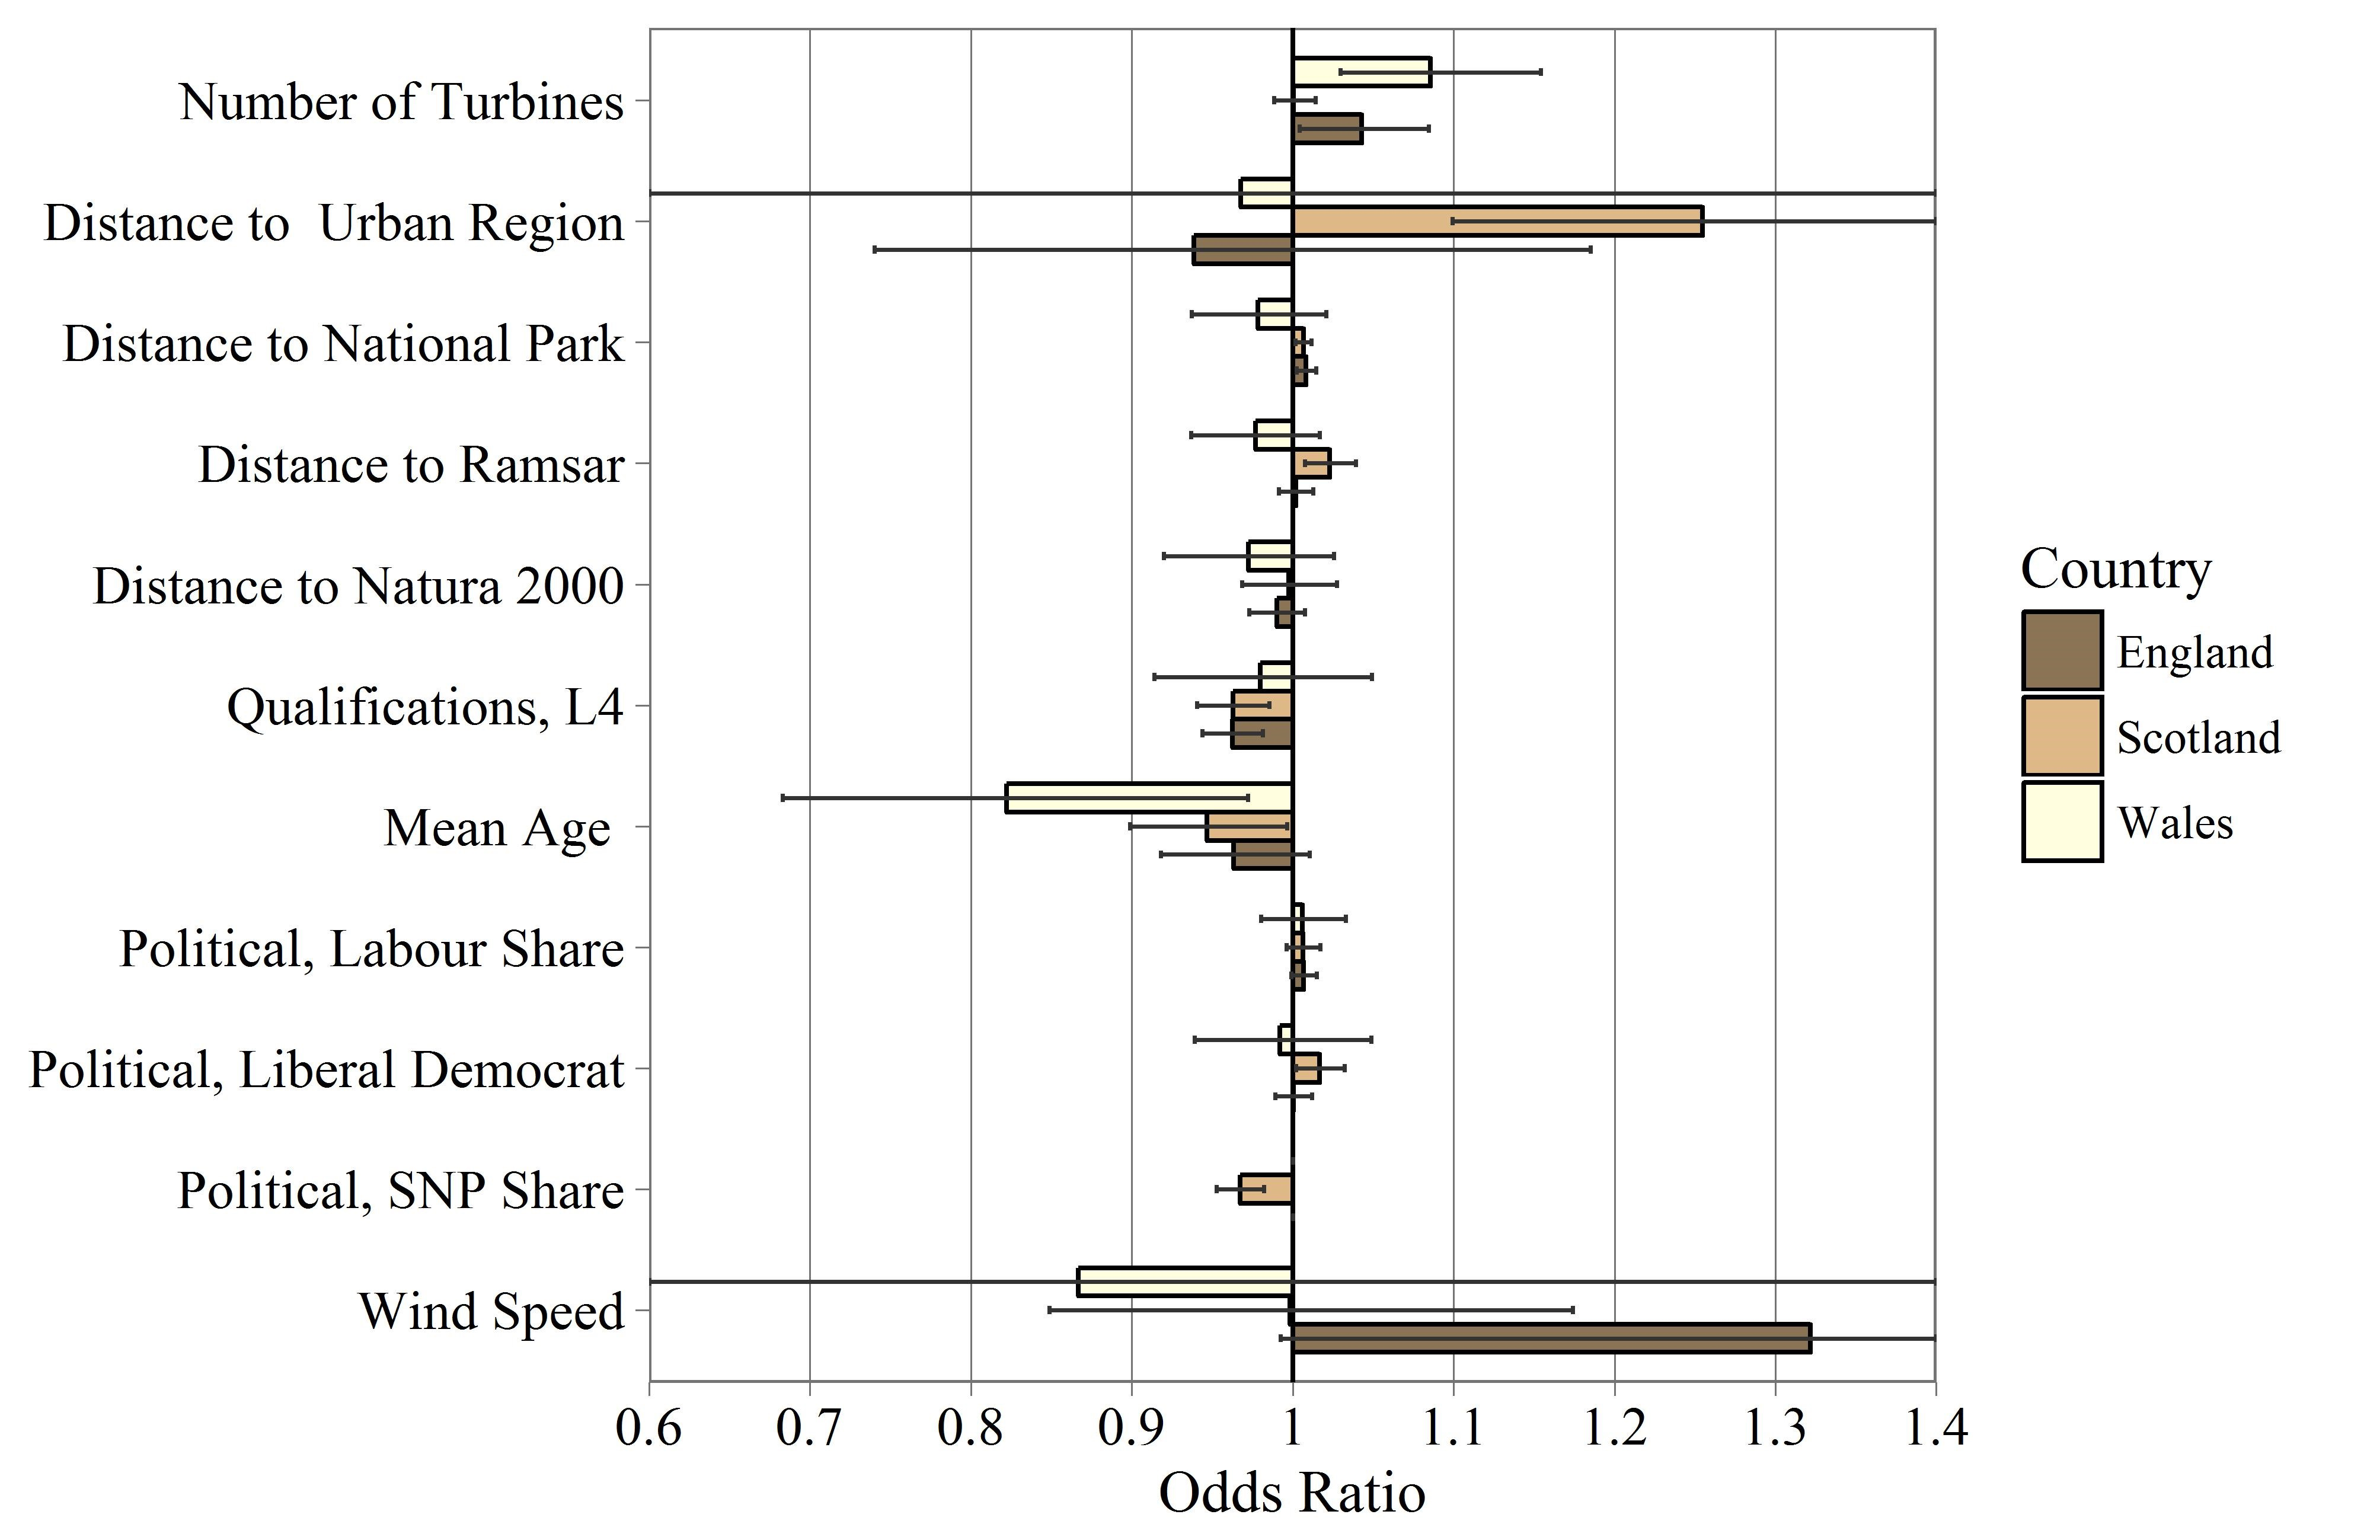
\includegraphics[width=8.8cm]{figures/OddsPlotSegmented} 

}

\caption{Odds plot for the nested logistic regression models for England, Scotland and Wales. Error bars indicate 95 confidence intervals.}\label{fig:OddsPlotSegmented}
\end{figure}

The results of the models are summarised in Table
\ref{tab:kableNestedModelResults}, which compares the two sets of split
data models compared against the results of the global parsimonious
model developed in Section \ref{ParameterRefinement}. There has been a
general increase in the fit of the models represented by the Nagelkirke
R\textsuperscript{2} values. For the Optimised parameter models, it can
be seen that the number of parameters within each model varies between
\texttt{min(num\_params)} and \texttt{max(num\_params)}, as derived from
the backward elimination process.

As the split models have been built using different datasets, there is
greater difficulty in directly comparing the diagnostics to assess the
model fit. Deviance, chi-sqared values, and residual deviance are all
dependent on the size of the datasets. Therefore, the models were
compared using the sum of the deviance of the split models, with values
of
\texttt{summary\_split\_model{[}"Deviance",2:4{]}\ \%\textgreater{}\%\ t\ \%\textgreater{}\%\ as.numeric\ \%\textgreater{}\%\ sum\ \%\textgreater{}\%\ round}
and
\texttt{summary\_split\_model{[}"Deviance",5:7{]}\ \%\textgreater{}\%\ t\ \%\textgreater{}\%\ as.numeric\ \%\textgreater{}\%\ sum\ \%\textgreater{}\%\ round}
for the \emph{Global} and \emph{Optimised} models respectively.

\begin{table}[!h]

\caption{\label{tab:kableNestedModelResults}Comparison of subset Logistic Regression Models based on the global parameters list}
\centering
\resizebox{\linewidth}{!}{\begin{tabular}[t]{llllllll}
\toprule
\multicolumn{2}{c}{ } & \multicolumn{3}{c}{Global Parameter} & \multicolumn{3}{c}{Optimised Parameters} \\
\cmidrule(l{2pt}r{2pt}){3-5} \cmidrule(l{2pt}r{2pt}){6-8}
X1 & Global & England & Scotland & Wales & England\_1 & Scotland\_1 & Wales\_1\\
\midrule
Observations & 1685 & 728 & 796 & 161 & 728 & 796 & 161\\
Parameters & 14 & 14 & 14 & 14 & 9 & 12 & 6\\
Deviance & 2079.34 & 884.02 & 957.03 & 199.97 & 888.86 & 959.0 & 205.42\\
R.n & 0.180 & 0.180 & 0.223 & 0.178 & 0.172 & 0.221 & 0.138\\
Chi Square & 244 & 105 & 146 & 23 & 100 & 144 & 18\\
\addlinespace
Degrees of Freedom & 13 & 13 & 13 & 13 & 8 & 11 & 5\\
p & 0.000 & 0.000 & 0.000 & 0.04092 & 0.000 & 0.000 & 0.00346\\
Residual Deviance & 1671 & 714 & 782 & 147 & 719 & 784 & 155\\
Accuracy & 33.5\% & 33.8\% & 32.8\% & 43.9\% & 33.4\% & 33.2\% & 40.6\%\\
\bottomrule
\end{tabular}}
\end{table}

\section{Discussion}\label{discussion}

\subsection{Significant Parameters}\label{significant-parameters}

Firstly, for project characteristics, the size of the turbine capacity
is indicated as a significant parameter, with larger turbines increasing
the chance of acceptance. This at first appears counter intuitive, but
may suggest that the developers of bigger turbines aremore likely to
appeal the decisions made against larger wind farms, as rejection of
such projects would result in a large loss of revenue. However, it
should be noted that this variable has a small standard deviation (sd =
1.0) compared to other variables included within this model, and
therefore the odds ratio inflates their influence within the model.

The distance to urban areas was indicated to be statistically
significant, although there is considerable uncertainty as indiciated by
the confidence interval. There are a number of potential causes for
this: firstly, it could indicate that high wind speed sites suitable for
development tend to be naturally less populated (i.e.~hilly, isolated
regions). Additionally, it may reflect a so-called ``Not in My Back
Yard'' (NIMBY) view from the vocal local population, with projects in
closer proximity to urban areas being more likely to be rejected. This
has been a relatively contentious subject within literature, with a
range of studies supporting
{[}\protect\hyperlink{ref-Haggett2006}{48},\protect\hyperlink{ref-Jones2010a}{62}{]}
and rejecting
{[}\protect\hyperlink{ref-Populus2005}{43},\protect\hyperlink{ref-Devine-Wright2005a}{45},\protect\hyperlink{ref-VanRensburg20}{49}{]}
the NIMBY argument. However this study provides quantitative evidence to
suggest that that sites closer to urban areas have a lower chance of
acceptance.

For landscape and environmental designations, distance to National
Parks, Ramsar and AONB were indicated as significant parameters although
have marginal impacts. This potentially reflects the negative visual
impacts which are often cited as a major impact of wind energy
developments
{[}\protect\hyperlink{ref-Langer2016}{32},\protect\hyperlink{ref-Jones2010a}{62}{]}.
However, it should be noted that these influences have a relatively low
impact, despite literature suggesting that landscape designations would
play a more important role.

The level of qualifications, and the mean age of the local populous have
been retained as significant parameters for demographic variables. It is
suggested that regions of higher education may be more effective in
organising campaign groups against such projects. This supports the
hypothesis developed by Van der Horst and Toke
{[}\protect\hyperlink{ref-VanderHorst2010}{23}{]} that developers were
\emph{``keen to avoid relatively privileged communities and target areas
where people are thought to less likely put up a fight''}. To the
author's knowledge, such a connection between acceptance rates and
demographics has not be previously quantitatively validated.

For political variables, the percentage of local council authority
control for Labour appear significant. While there is limited research
exploring political views and support for wind turbines, it had been
expected that there would be a level of correlation that may result from
the Conservative party, as their party has generally oppose the building
of wind turbines {[}\protect\hyperlink{ref-Smith2016}{63}{]}. In
addition, other studies have highlighted that voters of Labour and the
Liberal Democrats are personally more in favour of onshore wind
{[}\protect\hyperlink{ref-Populus2005}{43}{]}, which may result in less
local objection against projects in areas where they have stronger
support.

The analysis suggests that proximity to existing wind energy
developments may influence the likelihood of projects receiving
planning. The nearest operational wind energy project was indicated as
having a statistically significant negative effect, which suggests that
projects further away from an existing project are less likely to be
accepted. In addition, the nearest rejected project is suggested to be
have a negative estimate, inferring that the further the site is from a
previously rejected project, the higher the chance of acceptance. As
shown in Section \ref{AcceptanceParameters}, this ``proximity
hypothesis'' has been a contentious subject challenged within literature
{[}\protect\hyperlink{ref-Eltham2008}{36}--\protect\hyperlink{ref-Ladenburg2006}{38}{]}.
However, this study provides quantitative evidence to challenge this
view.

There are notable parameters which are frequently used in GIS modelling,
but do not prove influential, including wind speed and the proximity to
airports. This may reflect that these parameters represent technical
challenges which can be investigated in the early stages of project
development, and therefore any sites that are not suitable will not seek
planning permission.

\subsection{Model Perfomance}\label{model-perfomance}

As shown in Table 3, there is a relatively low level of fit with Psuedo
R2 values of 0.187.

\subsection{National Models}\label{national-models}

The split data model developed suggests that there are varying
influential parameters within England Scotland and Wales, although the
reduced number of observations used to build each model increases the
uncertainty substantially as indicated by the confidence intervals.
Parameters including \emph{Turbine Capacity}, \emph{Wind Speed} and
\emph{Distance to Urban Regions} show differing relationships for each
country. This suggests that there may be differing motives for projects
within each country as well as differential planning constraints. For
example, sites in England appear more sensitive to AONB and National
Parks than in Scotland and Wales, and supports research that national
level government decisions can influence the local developments
{[}\protect\hyperlink{ref-Langer2016}{32}{]}.

For the Scotland model, the percentage of local council authority
control for SNP appears significant, with increased percentage resulting
in a lower acceptance rate. However, upon further inspection, this was
deemed to be a potential confounding variable with the year of
application: SNP have increased their share of council seats between
1990 and 2016 from 15\% to 35\%, while at the same time the average
acceptance rates have reduced from around 75\% to 40\% across that
period. This parameter therefore appears to capture a national trend,
rather than highlighting any local political influences.

Splitting the model into England, Scotland and Wales marginally improved
these values to 0.11, 0.16 and 0.24, suggesting the model was a better
fit for Scotland and Wales. However, while the accuracy of the Scotland
model improved against the ``all countries'' model (60\% to 65\%), the
Wales only model has decreased to 57\%, suggesting that this model has
been overfitted due to the reduced number of observations (n = 132).

\section{Conclusions \& Implications}\label{conclusions-implications}

This paper has investigated the influence of geospatial, environmental,
demographic and political attributes on the probability of wind farm
planning approval in Great Britain between 1990 and 2016. The study
findings reveal that local demographic and political parameters appear
to influence the planning outcomes of projects, and that many of the
geospatial parameters typically integrated into wind turbine models
appear insignificant in determining site approval. To the authors'
knowledge, such quantitative findings have not previously been
demonstrated using such datasets.

It appears that certain demographics are less accepting of onshore wind
in Great Britain. Given that UK planning policy has now devolved power
locally and allowing local communities to have the final say on projects
{[}48{]}, there may be a clear block to development in certain regions
in the country.

In addition, the results raise concerns of the predictive ability of
existing geospatial modelling in locating wind energy sites. These
findings provide evidence to support existing literature that GIS tools
in themselves are of limited applicability
{[}\protect\hyperlink{ref-Malczewski2004}{22},\protect\hyperlink{ref-Toke2005}{44}{]},
and supports the conclusion that greater emphasis needs to be given to
the non-physical elements of a project (e.g.~Community engagement with
the scheme from an early stage)
{[}\protect\hyperlink{ref-Wolsink2000}{2},\protect\hyperlink{ref-Toke2008}{31},\protect\hyperlink{ref-Warren2010}{41}{]}.

Because of the low model fit, future work aims to integrate more
detailed information about specific wind turbine sites. It has not been
possible to include detailed information of the project development
within the analysis.

As highlighted within the literature, there have been recent changes in
legislation regarding the planning of wind energy. These grant greater
controls to local communities to oppose the development of wind turbines
{[}\protect\hyperlink{ref-Smith2016}{63}{]}. Such changes in planning
likely have an effect on the underlying influences of wind energy
acceptance rates, and therefore care is required forecasting the results
of a model based on historic data into future predictions. However, such
approaches still offer a useful insight for high-level regional
forecasting.

It should be noted that the parameters used to derive these findings are
obtained with context to Great Britain, and therefore may have limited
applicability internationally, and therefore should be applied with
caution outside of this region. There are opportunities to expand upon
this work by exploring the international context of the finding to widen
its applicability.

However, with the estimated cost of planning applications for commercial
scale projects exceeding \pounds 50000
{[}\protect\hyperlink{ref-RF2016}{64}{]}, there is large value in even
marginal improvements in the site selection. The findings from this
model can help inform regional level strategy and provide an insight to
developers of where projects may be more suitable for future development

POLICY

\subsection*{Acknowledgments}\label{acknowledgments}
\addcontentsline{toc}{subsection}{Acknowledgments}

This work is part of the activities of the Energy and Climate Change
Division and the Sustainable Energy Research Group at the University of
Southampton \url{www.energy.soton.ac.uk}. It is also supported by ESPRC
under grant EP/J017698/1, Transforming the Engineering of Cities to
Deliver Societal and Planetary Wellbeing and the Faculty of Engineering
and Environment at the University of Southampton.

\subsection*{Supplementary Files}\label{supplementary-files}
\addcontentsline{toc}{subsection}{Supplementary Files}

The full statistical analysis and turbine dataset is provided with the
analysis. The analysis and report was written using RMarkdown
{[}\protect\hyperlink{ref-R-rmarkdown}{65}{]}, and the original files
can be used to recreate the results presented in this report.

\section*{References}\label{references}
\addcontentsline{toc}{section}{References}

\hypertarget{refs}{}
\hypertarget{ref-UNEP2016}{}
{[}1{]} UNEP, Global trends in renewable energy, (2016).
\url{https://goo.gl/0GtPT4} (accessed January 20, 2017).

\hypertarget{ref-Wolsink2000}{}
{[}2{]} M. Wolsink, Wind power and the NIMBY-myth: institutional
capacity and the limited significance of public support, Renewable
Energy. 21 (2000) 49--64.
doi:\href{https://doi.org/10.1016/S0960-1481(99)00130-5}{10.1016/S0960-1481(99)00130-5}.

\hypertarget{ref-DECC2016}{}
{[}3{]} DECC, Renewable Energy Planing Data, (2016).
\url{https://www.gov.uk/government/collections/renewable-energy-planning-data}
(accessed April 25, 2016).

\hypertarget{ref-Voivontas1998}{}
{[}4{]} D. Voivontas, D. Assimacopoulos, a. Mourelatos, J. Corominas,
Evaluation of renewable energy potential using a GIS decision support
system, Renewable Energy. 13 (1998) 333--344.
doi:\href{https://doi.org/10.1016/S0960-1481(98)00006-8}{10.1016/S0960-1481(98)00006-8}.

\hypertarget{ref-Baban2001}{}
{[}5{]} S.M.J. Baban, T. Parry, Developing and applying a GIS-assisted
approach to locating wind farms in the UK, Renewable Energy. 24 (2001)
59--71.
doi:\href{https://doi.org/10.1016/S0960-1481(00)00169-5}{10.1016/S0960-1481(00)00169-5}.

\hypertarget{ref-Hansen2005}{}
{[}6{]} H.S. Hansen, GIS-based Multi-Criteria Analysis of Wind Farm
Development, Proceedings of the 10th Scandinavian Research Confrence on
Geographical Information Scient. (2005) 75--87.

\hypertarget{ref-Yue2006}{}
{[}7{]} C.D. Yue, S.S. Wang, GIS-based evaluation of multifarious local
renewable energy sources: A case study of the Chigu area of southwestern
Taiwan, Energy Policy. 34 (2006) 730--742.
doi:\href{https://doi.org/10.1016/j.enpol.2004.07.003}{10.1016/j.enpol.2004.07.003}.

\hypertarget{ref-Lee2009}{}
{[}8{]} A.H.I. Lee, H.H. Chen, H.Y. Kang, Multi-criteria decision making
on strategic selection of wind farms, Renewable Energy. 34 (2009)
120--126.
doi:\href{https://doi.org/10.1016/j.renene.2008.04.013}{10.1016/j.renene.2008.04.013}.

\hypertarget{ref-Janke2010}{}
{[}9{]} J.R. Janke, Multicriteria GIS modeling of wind and solar farms
in Colorado, Renewable Energy. 35 (2010) 2228--2234.
\href{http://people.umass.edu/bethanyb/Janke,\%202010.pdf}{http://people.umass.edu/bethanyb/Janke, 2010.pdf}.

\hypertarget{ref-SQWEnergy2010}{}
{[}10{]} SQW Energy, Renewable and Low-carbon Energy Capacity
Methodology Methodology for the English Regions, 2010.

\hypertarget{ref-Aydin2010}{}
{[}11{]} N.Y. Aydin, E. Kentel, S. Duzgun, GIS-based environmental
assessment of wind energy systems for spatial planning: A case study
from Western Turkey, Renewable and Sustainable Energy Reviews. 14 (2010)
364--373.
doi:\href{https://doi.org/10.1016/j.rser.2009.07.023}{10.1016/j.rser.2009.07.023}.

\hypertarget{ref-VanHaaren2011}{}
{[}12{]} R. Van Haaren, V. Fthenakis, GIS-based wind farm site selection
using spatial multi-criteria analysis (SMCA): Evaluating the case for
New York State, Renewable and Sustainable Energy Reviews. 15 (2011)
3332--3340.
doi:\href{https://doi.org/10.1016/j.rser.2011.04.010}{10.1016/j.rser.2011.04.010}.

\hypertarget{ref-Sliz-Szkliniarz2011}{}
{[}13{]} B. Sliz-Szkliniarz, J. Vogt, GIS-based approach for the
evaluation of wind energy potential: A case study for the
Kujawsko-Pomorskie Voivodeship, Renewable and Sustainable Energy
Reviews. 15 (2011) 1696--1707.
doi:\href{https://doi.org/10.1016/j.rser.2010.11.045}{10.1016/j.rser.2010.11.045}.

\hypertarget{ref-Gass2013}{}
{[}14{]} V. Gass, J. Schmidt, F. Strauss, E. Schmid, Assessing the
economic wind power potential in Austria, Energy Policy. 53 (2013)
323--330.
doi:\href{https://doi.org/10.1016/j.enpol.2012.10.079}{10.1016/j.enpol.2012.10.079}.

\hypertarget{ref-Neufville2013}{}
{[}15{]} L. Neufville, Wind farm Site Suitability Selection using
Multi-Criteria Analysis (MCA) and Spatial Modelling, (2013) 1--29.

\hypertarget{ref-Miller2014}{}
{[}16{]} A. Miller, R. Li, A Geospatial Approach for Prioritizing Wind
Farm Development in Northeast Nebraska, USA, ISPRS International Journal
of Geo-Information. 3 (2014) 968--979.
doi:\href{https://doi.org/10.3390/ijgi3030968}{10.3390/ijgi3030968}.

\hypertarget{ref-Wang2014}{}
{[}17{]} Q. Wang, M.M. M'Ikiugu, I. Kinoshita, A GIS-based approach in
support of spatial planning for renewable energy: A case study of
Fukushima, Japan, Sustainability (Switzerland). 6 (2014) 2087--2117.
doi:\href{https://doi.org/10.3390/su6042087}{10.3390/su6042087}.

\hypertarget{ref-Watson2015}{}
{[}18{]} J.J.W. Watson, M.D. Hudson, Regional Scale wind farm and solar
farm suitability assessment using GIS-assisted multi-criteria
evaluation, Landscape and Urban Planning. 138 (2015) 20--31.
doi:\href{https://doi.org/10.1016/j.landurbplan.2015.02.001}{10.1016/j.landurbplan.2015.02.001}.

\hypertarget{ref-Noorollahi2015}{}
{[}19{]} Y. Noorollahi, H. Yousefi, M. Mohammadi, Multi-criteria
decision support system for wind farm site selection using GIS,
Sustainable Energy Technologies and Assessments. 13 (2015) 38--50.
doi:\href{https://doi.org/10.1016/j.seta.2015.11.007}{10.1016/j.seta.2015.11.007}.

\hypertarget{ref-Atici2015}{}
{[}20{]} K.B. Atici, A.B. Simsek, A. Ulucan, M.U. Tosun, A GIS-based
Multiple Criteria Decision Analysis approach for wind power plant site
selection, Utilities Policy. 37 (2015) 86--96.
doi:\href{https://doi.org/10.1016/j.jup.2015.06.001}{10.1016/j.jup.2015.06.001}.

\hypertarget{ref-Baseer2017}{}
{[}21{]} M. Baseer, S. Rehman, J. Meyer, M.M. Alam, GIS-based site
suitability analysis for wind farm development in Saudi Arabia, Energy.
(2017).
doi:\href{https://doi.org/10.1016/j.energy.2017.10.016}{10.1016/j.energy.2017.10.016}.

\hypertarget{ref-Malczewski2004}{}
{[}22{]} J. Malczewski, GIS-based land-use suitability analysis: A
critical overview, Progress in Planning. 62 (2004) 3--65.
doi:\href{https://doi.org/10.1016/j.progress.2003.09.002}{10.1016/j.progress.2003.09.002}.

\hypertarget{ref-VanderHorst2010}{}
{[}23{]} D. van der Horst, D. Toke, Exploring the landscape of wind farm
developments; local area characteristics and planning process outcomes
in rural England, Land Use Policy. 27 (2010) 214--221.
doi:\href{https://doi.org/10.1016/j.landusepol.2009.05.006}{10.1016/j.landusepol.2009.05.006}.

\hypertarget{ref-Cirucci2014}{}
{[}24{]} J. Cirucci, Retrospective GIS-Based Multi-Criteria Decision
Analysis, (2014).

\hypertarget{ref-Brody2002}{}
{[}25{]} J.G. Brody, D.J. Vorhees, S.J. Melly, S.R. Swedis, P.J. Drivas,
R.A. Rudel, Using GIS and historical records to reconstruct residential
exposure to large-scale pesticide application, Journal of Exposure
Analysis and Environmental Epidemiology. 12 (2002) 64--80.
doi:\href{https://doi.org/10.1038/sj/jea/7500205}{10.1038/sj/jea/7500205}.

\hypertarget{ref-Mohamed2004}{}
{[}26{]} N.S. Mohamed, L.M. Nofal, M.H.A. Hassan, S.M. Elkaffas,
Geographic information systems (GIS) analysis of under five mortality in
Alexandria., The Journal of the Egyptian Public Health Association. 79
(2004) 243--262.

\hypertarget{ref-Yamada2009}{}
{[}27{]} I. Yamada, P.A. Rogerson, G. Lee, GeoSurveillance: A GIS-based
system for the detection and monitoring of spatial clusters, Journal of
Geographical Systems. 11 (2009) 155--173.
doi:\href{https://doi.org/10.1007/s10109-009-0080-1}{10.1007/s10109-009-0080-1}.

\hypertarget{ref-Garcia-Ayllon2013}{}
{[}28{]} S. Garcia-Ayllon, Retrospective analysis of urban development
in the Spanish Mediterranean coast, WIT Transactions on Ecology and the
Environment. 179 VOLUME (2013) 291--302.
doi:\href{https://doi.org/10.2495/SC130251}{10.2495/SC130251}.

\hypertarget{ref-USEPA2002}{}
{[}29{]} O.O. of R.C. US EPA, Recovery, Waste Transfer Stations: A
Manual for Decision-Making, (2002) 1--66.
\url{papers3://publication/uuid/7CAEDFA2-1B14-4CFF-8B13-1E920D35AD80}.

\hypertarget{ref-Cirucci2015}{}
{[}30{]} J.F. Cirucci, D.A. Miller, J.I. Blanford, Retrospective
GIS-Based Multi-Criteria Decision Analysis: A Case Study of California
Waste Transfer Station Siting Decisions, Proceedings of the
International Symposium on Sustainable Systems and Technologies. 3
(2015).
doi:\href{https://doi.org/10.6084/m9.figshare.1512514}{10.6084/m9.figshare.1512514}.

\hypertarget{ref-Toke2008}{}
{[}31{]} D. Toke, S. Breukers, M. Wolsink, Wind power deployment
outcomes: How can we account for the differences?, Renewable and
Sustainable Energy Reviews. 12 (2008) 1129--1147.
doi:\href{https://doi.org/10.1016/j.rser.2006.10.021}{10.1016/j.rser.2006.10.021}.

\hypertarget{ref-Langer2016}{}
{[}32{]} K. Langer, T. Decker, J. Roosen, K. Menrad, A qualitative
analysis to understand the acceptance of wind energy in Bavaria,
Renewable and Sustainable Energy Reviews. 64 (2016) 248--259.
doi:\href{https://doi.org/10.1016/j.rser.2016.05.084}{10.1016/j.rser.2016.05.084}.

\hypertarget{ref-Devine-Wright2005}{}
{[}33{]} P. Devine-Wright, Local aspects of UK renewable energy
development: exploring public beliefs and policy implications, Local
Environment. 10 (2005) 57--69.
doi:\href{https://doi.org/10.1080/1354983042000309315}{10.1080/1354983042000309315}.

\hypertarget{ref-Warren2005}{}
{[}34{]} 'Green On Green': Public perceptions of wind power in Scotland
and Ireland, Journal of Environmental Planning and Management. 48 (2005)
853--875.
doi:\href{https://doi.org/10.1080/09640560500294376}{10.1080/09640560500294376}.

\hypertarget{ref-Krohn1999}{}
{[}35{]} S. Krohn, S. Damborg, On Public Attitudes Towards Wind Power,
Renewable Energy. 16 (1999) 954--960.
doi:\href{https://doi.org/10.1016/S0960-1481(98)00339-5}{10.1016/S0960-1481(98)00339-5}.

\hypertarget{ref-Eltham2008}{}
{[}36{]} D.C. Eltham, G.P. Harrison, S.J. Allen, Change in public
attitudes towards a Cornish wind farm: Implications for planning, Energy
Policy. 36 (2008) 23--33.
doi:\href{https://doi.org/10.1016/j.enpol.2007.09.010}{10.1016/j.enpol.2007.09.010}.

\hypertarget{ref-Meyerhoff2010}{}
{[}37{]} J. Meyerhoff, C. Ohl, V. Hartje, Landscape externalities from
onshore wind power, Energy Policy. 38 (2010) 82--92.
doi:\href{https://doi.org/10.1016/j.enpol.2009.08.055}{10.1016/j.enpol.2009.08.055}.

\hypertarget{ref-Ladenburg2006}{}
{[}38{]} J. Ladenburg, A. Dubgaard, Willingness To Pay For Reduced
Visual Disamenities From Off-Shore Wind Farms In Denmark BT - Third
World Congress Of Environmental And Resource Economists, (2006).

\hypertarget{ref-Strachan2004}{}
{[}39{]} P.a. Strachan, D. Lal, Wind energy policy, planning and
management practice in the UK: Hot air or a gathering storm?, Regional
Studies. 38 (2004) 551--571.
doi:\href{https://doi.org/10.1080/0143116042000229311}{10.1080/0143116042000229311}.

\hypertarget{ref-Jones2011}{}
{[}40{]} C.R. Jones, B.J. Orr, J.R. Eiser, When is enough, enough?
Identifying predictors of capacity estimates for onshore wind-power
development in a region of the UK, Energy Policy. 39 (2011) 4563--4577.
doi:\href{https://doi.org/10.1016/j.enpol.2011.04.044}{10.1016/j.enpol.2011.04.044}.

\hypertarget{ref-Warren2010}{}
{[}41{]} C.R. Warren, M. McFadyen, Does community ownership affect
public attitudes to wind energy? A case study from south-west Scotland,
Land Use Policy. 27 (2010) 204--213.
doi:\href{https://doi.org/10.1016/j.landusepol.2008.12.010}{10.1016/j.landusepol.2008.12.010}.

\hypertarget{ref-Devine-Wright2007}{}
{[}42{]} P. Devine-Wright, Reconsidering public attitudes and public
acceptance of renewable energy technologies : a critical review,
Architecture. Working Pa (2007) 1--15. \url{goo.gl/wdj68L}.

\hypertarget{ref-Populus2005}{}
{[}43{]} Populus, Energy Balance of Power Poll Fieldwork : July 1st-6th
2005, (2005) 1--23.

\hypertarget{ref-Toke2005}{}
{[}44{]} D. Toke, Explaining wind power planning outcomes: Some findings
from a study in England and Wales, Energy Policy. 33 (2005) 1527--1539.
doi:\href{https://doi.org/10.1016/j.enpol.2004.01.009}{10.1016/j.enpol.2004.01.009}.

\hypertarget{ref-Devine-Wright2005a}{}
{[}45{]} P. Devine-Wright, Beyond NIMBYism: Towards an integrated
framework for understanding public perceptions of wind energy, Wind
Energy. 8 (2005) 125--139.
doi:\href{https://doi.org/10.1002/we.124}{10.1002/we.124}.

\hypertarget{ref-Wustenhagen2007}{}
{[}46{]} R. Wustenhagen, M. Wolsink, M.J. Burer, Social acceptance of
renewable energy innovation: An introduction to the concept, Energy
Policy. 35 (2007) 2683--2691.
doi:\href{https://doi.org/10.1016/j.enpol.2006.12.001}{10.1016/j.enpol.2006.12.001}.

\hypertarget{ref-Sonnberger2017}{}
{[}47{]} M. Sonnberger, M. Ruddat, Local and socio-political acceptance
of wind farms in Germany, Technology in Society. 51 (2017) 56--65.
doi:\href{https://doi.org/10.1016/j.techsoc.2017.07.005}{10.1016/j.techsoc.2017.07.005}.

\hypertarget{ref-Haggett2006}{}
{[}48{]} C. Haggett, D. Toke, Crossing the great divide-using
multi-method analysis to understand opposition to windfarms, Public
Administration. 84 (2006) 103--120.
doi:\href{https://doi.org/10.1111/j.0033-3298.2006.00495.x}{10.1111/j.0033-3298.2006.00495.x}.

\hypertarget{ref-VanRensburg20}{}
{[}49{]} T.M. van Rensburg, H. Kelley, N. Jeserich, What influences the
probability of wind farm planning approval: Evidence from Ireland,
Ecological Economics. 111 (2015) 12--22.
doi:\href{https://doi.org/10.1016/j.ecolecon.2014.12.012}{10.1016/j.ecolecon.2014.12.012}.

\hypertarget{ref-HMGovernment2014}{}
{[}50{]} HM Government, Planning Portal Northern Ireland, (2014).

\hypertarget{ref-DTI2001}{}
{[}51{]} DTI, NOABL Windspeed Database, (2001).
\url{https://goo.gl/6BALyv} (accessed October 21, 2016).

\hypertarget{ref-Survey2016}{}
{[}52{]} Ordnance Survey, OS Strategi, (2016).
\url{https://data.gov.uk/dataset/strategi}.

\hypertarget{ref-Overpass2016}{}
{[}53{]} OSM, Overpass API, (2016). \url{https://overpass-turbo.eu/}.

\hypertarget{ref-Pope2017}{}
{[}54{]} A. Pope, UK National Parks, (2017).
\url{http://dx.doi.org/10.7488/ds/1810}.

\hypertarget{ref-Commission2015}{}
{[}55{]} European Commission, Digital Elevation Model over Europe
(EU-DEM), (2015).
\href{http://www.eea.europa.eu/data-and-maps/data/eu-dem\%7B/\#\%7Dtab-european-data}{http://www.eea.europa.eu/data-and-maps/data/eu-dem\{\textbackslash{}\#\}tab-european-data}
(accessed November 20, 2016).

\hypertarget{ref-Fleming1979}{}
{[}56{]} M.D. Fleming, R.M. Hoffer, Machine Processing of Landsat MSS
Data and DMA Topographic Data for Forest Cover Type Mapping, LARS
Technical Report 082879 Laboratory for Applications of Remote Sensing,
Purdue University, West Lafayette, Indiana. (1979) 377--390.

\hypertarget{ref-OfficeforNationalStatistics}{}
{[}57{]} Office for National Statistics, 2011 Census data, (2016).
\url{https://www.ons.gov.uk/census/2011census/2011censusdata} (accessed
October 20, 2016).

\hypertarget{ref-Harrell2001}{}
{[}58{]} F.E. Harrell, Regression modeling strategies. With applications
to linear models, logistic regression, and survival analysis, 2001.
doi:\href{https://doi.org/10.1007/978-1-4757-3462-1}{10.1007/978-1-4757-3462-1}.

\hypertarget{ref-Hosmer2004}{}
{[}59{]} D.W. Hosmer, S. Lemeshow, Applied Logistic Regression Second
Edition, 2004.
doi:\href{https://doi.org/10.1002/0471722146}{10.1002/0471722146}.

\hypertarget{ref-ONS2013}{}
{[}60{]} ONS, 2011 Census, Quick Statistics for Wales on National
Identity, Passports Held and Country of Birth, (2013).

\hypertarget{ref-Ward2008}{}
{[}61{]} M.D. Ward, Spatial Regression Models, 2008.

\hypertarget{ref-Jones2010a}{}
{[}62{]} C.R. Jones, J. Richard Eiser, Understanding 'local' opposition
to wind development in the UK: How big is a backyard?, Energy Policy. 38
(2010) 3106--3117.
doi:\href{https://doi.org/10.1016/j.enpol.2010.01.051}{10.1016/j.enpol.2010.01.051}.

\hypertarget{ref-Smith2016}{}
{[}63{]} L. Smith, Planning for onshore wind farms, House of Commons
Briefing Paper. (2016).
\url{http://www.parliament.uk/briefing-papers/sn04370.pdf}.

\hypertarget{ref-RF2016}{}
{[}64{]} Renewables First, Wind Turbine Planning Permission, (2016).
\url{http://www.renewablesfirst.co.uk/windpower/wind-turbine-consenting/wind-turbine-planning-permission/}
(accessed September 2, 2017).

\hypertarget{ref-R-rmarkdown}{}
{[}65{]} J. Allaire, Y. Xie, J. McPherson, J. Luraschi, K. Ushey, A.
Atkins, H. Wickham, J. Cheng, W. Chang, Rmarkdown: Dynamic documents for
r, 2017. \url{https://CRAN.R-project.org/package=rmarkdown}.

\newpage

\section*{Appendix}\label{appendix}
\addcontentsline{toc}{section}{Appendix}

\begin{landscape}\begin{table}

\caption{\label{tab:unnamed-chunk-2}Summary of data sources used within model}
\centering
\resizebox{\linewidth}{!}{\begin{tabular}[t]{rlllllll}
\toprule
ID & Category & Variable & Source & Data Type & Variable Value & Value Type & Unit\\
\midrule
1 & Turbine & Wind Turbine Planning Data & REPD & Tabular & Planning Outcome & Categorical & Accept/Reject\\
2 &  & Turbine Capacity &  & Tabular & Megawatts/turbine & Continuous & MW\\
3 &  & Number of Turbines &  & Tabular &  & Continuous & \\
4 &  & Year &  & Tabular &  & Discrete & \\
5 &  & Country &  & Tabular &  & Categorical & \\
\addlinespace
6 & Resource & Wind Speed & NOABL & Raster & Annualised Wind Speed & Continuous & m/s\\
7 & Features & Airports & OpenGeo & Points & Distance to Feature & Continuous & km\\
8 &  & Roads\textsuperscript{a} & OS Strategi & Lines & Distance to Feature & Continuous & km\\
9 &  & Railways &  & Lines & Distance to Feature & Continuous & km\\
10 &  & Urban Areas &  & Polygons & Distance to Feature & Continuous & km\\
\addlinespace
11 &  & HV Powerlines\textsuperscript{b} &  & Lines & Distance to Feature & Continuous & km\\
12 & Landscape & Areas of Outstanding Natural Beauty & National Heritage & Polygons & Distance to Feature & Continuous & km\\
13 &  & National Parks &  & Polygons & Distance to Feature & Continuous & km\\
14 &  & Heritage Coast &  & Polygons & Distance to Feature & Continuous & km\\
15 & Nature & Special Protection Areas &  & Polygons & Distance to Feature & Continuous & km\\
\addlinespace
16 &  & National Nature Reserve &  & Polygons & Distance to Feature & Continuous & km\\
17 &  & Sites of Special Scientific Interest &  & Polygons & Distance to Feature & Continuous & km\\
18 &  & Special Areas of Conservation &  & Polygons & Distance to Feature & Continuous & km\\
19 & Geographic & Elevation & EU DEM & Raster & Height above sea level & Integer & m\\
20 &  & Slope & Derived from 18 & Raster & Gradient & Continuous & \%\\
\addlinespace
21 & Census & Level of Qualification\textsuperscript{c} & ONS & Tabular & Higher than L4 & Continuous & \%\\
22 &  & Age &  & Tabular & Mean & Continuous & Years\\
23 &  & Social Grade\textsuperscript{d} &  & Tabular & Social Grade AB & Continuous & \%\\
24 &  & Tenure &  & Tabular & Home Ownership & Continuous & \%\\
25 & Political & Conservatives & Populus & Tabular & Percentage of Council & Continuous & \%\\
\addlinespace
26 &  & Labour &  & Tabular & Percentage of Council & Continuous & \%\\
27 &  & Liberal Democrat &  & Tabular & Percentage of Council & Continuous & \%\\
28 & Proximity & Nearest Turbine (Operational) & Calculated & Points & Distance to Turbine & Continuous & km\\
29 &  & Nearest Turbine (Rejected) & Calculated & Points & Distance to Turbine & Continuous & km\\
\bottomrule
\multicolumn{8}{l}{\textsuperscript{a} Roads are broken into four main categories: Motorways, A Roads, B Roads and Minor Roads}\\
\multicolumn{8}{l}{\textsuperscript{b} High Voltage network at 140 400kV}\\
\multicolumn{8}{l}{\textsuperscript{c} L4 represents degree level or above}\\
\multicolumn{8}{l}{\textsuperscript{d} AB represents Higher and intermediate managerial, administrative, professional occupation}\\
\end{tabular}}
\end{table}
\end{landscape}


\end{document}
